\mynewpage
\chapter{Algebraic Geometry}\label{sec:algebraic:geometry}

\indraftnote{Some of this material goes into the main book. Here we're just
putting all our notes in}

\indraftnote{This is getting into shape but is waaay behind what we have in other documents.}

\section{Computational Aspects}

\section{David Pinho's MSc.\ Notes}
Esta seção se destina a apresentar um resumo das definições básicas em Geometria Algébrica, bem como alguns conceitos e definições mais avançados necessários ao entendimento do procedimento de solução de sistemas de equações polinomiais. Para acessar um detalhamento maior da teoria juntamente com as demonstrações dos teoremas, o leitor pode consultar os livros Cox et al. (2005) e Cox et al. (2007).

\subsection{Definições básicas}

A Geometria Algébrica tem como objetivo principal de estudos as variedades algébricas, os objetos geométricos
formados pelos pontos que são soluções de um sistema de equações polinomiais. Para realizar esse estudo, utiliza técnicas de álgebra comutativa em conjunto com a linguagem geométrica.

{\it Monômios} são o produto de $n$ variáveis da forma $x_1^{\alpha_1}\cdot x_2^{\alpha_2} \cdot ... \cdot x_n^{\alpha_n}$ onde os expoentes são números inteiros não-negativos. O grau total de um monômio é a soma dos expoentes das variáveis e é denotado por $|\alpha|=\alpha_1+\alpha_2+...+\alpha_n$, e para simplificar a notação é adotada a convenção onde $\alpha=(\alpha_1,\alpha_2,...,\alpha_n)$ é o vetor dos expoentes e $x^\alpha=x_1^{\alpha_1}\cdot x_2^{\alpha_2} \cdot ... \cdot x_n^{\alpha_n}$ é a representação do monômio.

{\it Polinômios} são combinações lineares dos monômios denotados por
\begin{equation*}
f=\sum_\alpha a_\alpha x^\alpha,\quad\text{onde}\quad a_\alpha\in k.
\end{equation*} 
Os coeficientes desses polinômios pertencem a um conjunto numérico denominado {\it corpo}, denotado por $k$, que pode ser o conjunto dos números complexos ou reais, por exemplo. Informalmente, corpo é um conjunto fechado para adição, subtração, multiplicação e divisão com suas propriedades usuais. O conjunto de todos os polinômios nas $n$ variáveis definidas num corpo $k$ é denotado por $k[x_1,...,x_n]$.

Se estivermos trabalhando com pouca variáveis podemos utilizar $x$, $y$ e $z$ e como exemplo temos
\begin{equation*}
f=2x^3y^2z+\frac{2}{3}y^3z^3-3xyz+y^2\quad\in\quad\mathbb{Q}[x,y,z],
\end{equation*} 
onde
\begin{itemize}
\item os {\it coeficientes} são 2, $\frac{2}{3}$, -3 e 1,
\item os {\it termos} são cada monômio junto com o respectivo coeficiente
\item o {\it grau total} do polinômio é o grau do monômio de maior grau; no caso temos dois monômios com grau 6.
\end{itemize}

A soma e o produto de dois polinômios também são polinômios, mas um polinômio $f$ divide um polinômio $g$ apenas se existe um polinômio $h$ onde $g=f\,h$. Assim, entre polinômios ficam satisfeitos os axiomas de adição e multiplicação em um corpo, mas não a existência de um inverso multiplicativo, pois por exemplo, $f=\frac{1}{x}$ não é um polinômio. Os elementos que obedecem essa estrutura formam um {\it anel comutativo}, com estudos feitos com base na {\it álgebra comutativa}, e por isso o conjunto $k[x_1,...,x_n]$ é chamado {\it anel de polinômios}.

\subsection{Ideal e variedade}
Um espaço $n$-dimensional num corpo $k$ é definido como
\begin{equation*}
k^n=\{(a_1,...,a_n)\,/\, a_1,...,a_n\in k\},
\end{equation*}
e é possível relacionar polinômios com um espaço $n$-dimensional observando que um polinômio nos dá uma função
\begin{equation*}
f:k^n\rightarrow k\quad\text{com}\quad f=\sum_\alpha a_\alpha x^\alpha\quad \in\quad k[x_1,...,x_n].
\end{equation*}
A capacidade em tratar polinômios como funções é o que possibilita ligar álgebra e geometria através das chamadas {\it variedades}, definida a seguir e denotada por ${\bf V}$.
\begin{equation*}
{\bf V}(f_1,...,f_s)=\{(a_1,...,a_n)\in k^n/\, f_i(a_1,...,a_n)=0, \,\forall\,\, 1\le i\le s\}.
\end{equation*}
Portanto, variedades podem ser entendidas como o conjunto de vetores que são solução de um sistema de equações polinomiais, e que fornecem uma representação geométrica para a solução do sistema sempre que possível.

Como exemplo, temos na Figura \ref{fig.variedades} a representação geométrica das variedades ${\bf V}(xy-x^3+1)$ e ${\bf V}(-x^2-y+z)$, onde cada ponto no plano e no espaço é representado pelas soluções de $xy-x^3+1=0$ e $-x^2-y+z=0$, respectivamente.
\begin{figure}
\caption{Variedades.}
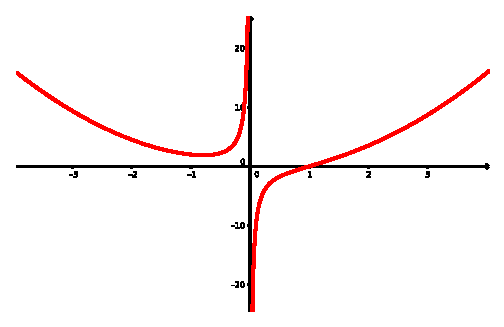
\includegraphics[width=.57\hsize]{variedade-1}\hfill
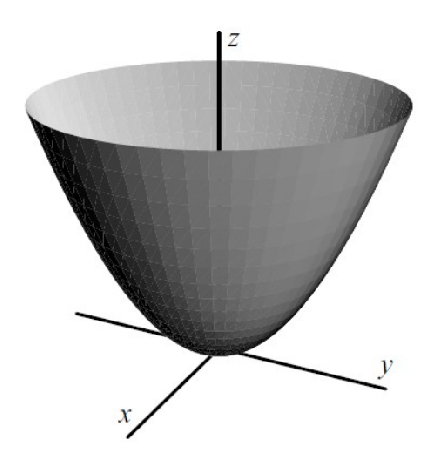
\includegraphics[width=.4\hsize]{variedade-3D}\hfill
\legend{As representações geométricas podem ser obtidas usando as funções ({\tt a}) $y=\frac{x^3-1}{x}$ e ({\tt b}) $z=x^2+y$.}
\source{({\tt a}) O autor. ({\tt b}) Cox et al. (2005).}
\label{fig.variedades}
\end{figure} 

{\it Ideal} é um subconjunto de $k[x_1,...,x_n]$ denotado por $I$ que satisfaz as condições:
\begin{itemize}
\item $0\in I$;
\item $f,g\,\in I \Rightarrow (f+g)\in I$;
\item $f \in I$ e $h \in k[x_1,...,x_n] \Rightarrow h\,f \in I$. 
\end{itemize}

Se $f_1,...,f_s$ são polinômios em $k[x_1,...,x_n]$ então podemos definir um ideal através desses polinômios que são chamados de {\it base} do ideal, usando a notação
\begin{equation*}
I=\left\langle f_1,...,f_s \right\rangle = \{\sum_{i=1}^s h_if_i\,:\,h_1,...,h_s \in k[x_1,...,x_n]\}.
\end{equation*}
Por exemplo, para sabermos se o polinômio $x^2-2x+2-y$ pertence ao ideal $\left\langle x-1-t\,,\,y-1-t^2 \right\rangle$ devemos verificar se é possível escrevê-lo como combinação das bases desse ideal, 
\begin{equation*}
x^2-2x+2-y=(x-1+t)(x-1-t)+(-1)(y-1-t^2).
\end{equation*}
Um mesmo ideal pode ser formado por bases diferentes e, quando isso acontece, as variedades definidas por cada base também são iguais, ou seja
\begin{equation*}
\left\langle f_1,...,f_s \right\rangle = \left\langle g_1,...,g_s \right\rangle \Rightarrow {\bf V}(f_1,...,f_s)={\bf V}(g_1,...,g_s).
\end{equation*}
Por exemplo, temos a seguir um ideal formado por bases diferentes (podemos verificar que se trata do mesmo ideal escrevendo os polinômios da esquerda como combinação dos polinômios da direita e reciprocamente) e que possuem variedades iguais:
\begin{equation*}
\left\langle 2x^2+3y^2-11\,,\,x^2-y^2-3 \right\rangle = \left\langle x^2-4\,,\,y^2-1 \right\rangle,\,\, \text{logo}
\end{equation*}
\begin{equation}\label{eq.variedades}
{\bf V}(2x^2+3y^2-11\,,\,x^2-y^2-3)={\bf V}(x^2-4\,,\,y^2-1)=\{(\pm2,\pm1)\}.
\end{equation}
Observe que todos os polinômios de um ideal terão o mesmo conjunto variedade gerado pelos polinômios da base. Observe ainda, que a base de um ideal pode ser pensada como um sistema de equações polinomiais, e que para encontrarmos o conjunto solução do sistema (variedade) podemos converter a base dada numa base mais simples conforme a relação \ref{eq.variedades}. Mais à frente veremos que é exatamente esse o procedimento realizado pelas bases de Gr\"obner.

\subsection{As bases de Gr\"obner}

Para sabermos se um polinômio $f$ pertence a um ideal devemos dividir $f$ pelas bases do ideal e verificar se o resto é zero, pois assim $f$ pode ser escrito como combinação dos polinômios da base. Na divisão de polinômios de uma variável o resto é único, mas para polinômios de mais de uma variável, tanto o resto como os quocientes podem variar dependendo da ordem dos divisores e da ordenação de monômios escolhida ({\it lexicográfica, lexicográfica graduada e lexicográfica graduada reversa}). Para detalhes sobre divisão de polinômios de várias variáveis consultar Cox et al. (2005). 

Por exemplo, vamos verificar se o polinômio $f=xy^2-x$ pertence ao ideal $I=\left\langle xy+1\,,\,y^2-1 \right\rangle$. Efetuando a divisão de $f$ por $\{xy+1\,,\,y^2-1\}$ nesta ordem, obtemos
\begin{equation*}
xy^2-x=y(xy+1)+0(y^2-1)+(-x-y)
\end{equation*}  
com resto $-x-y$. Mas efetuando a divisão na ordem $\{y^2-1\,,\,xy+1\}$ teremos
\begin{equation*}
xy^2-x=x(y^2-1)+0(xy+1)+0
\end{equation*} 
com resto zero. Assim, $f\in I$ e vemos que, dada uma base qualquer de $I$, o resto zero é uma condição suficiente para que $f\in I$ mas não é uma condição necessária. 

Precisamos de uma base que facilite verificar se um polinômio pertence a um ideal, e as bases de Gr\"obner tem essa propriedade, pois um polinômio $f$ quando dividido pelas bases de Gr\"obner deixa resto único, não importanto a ordem dos divisores (base do ideal). Assim, sendo $G=\{g_1,...,g_t\}$ uma base de Gr\"obner, então 
\begin{equation*}
f\in I \Leftrightarrow \text{o resto da divisão de $f$ por $G$ é zero}.
\end{equation*}
Essa propriedade é tão importante que às vezes é tomada como a própria definição para as bases de Gr\"obner. O resto da divisão de um polinômio $f$ por $G=\{g_1,...,g_t\}$ é denotado por $\overline{f}^G$. Por exemplo, dividindo $f=x^5y$ por $G=\{x^2y-y^2\,,\,x^4y^2-y^2\}$ é $\overline{x^5y}^G=xy^3$, pois
\begin{equation*}
x^5y=(x^3+xy)(x^2y-y^2)+(0)(x^4y^2-y^2)+xy^3.
\end{equation*}
Para verificarmos se uma base é uma base de Gr\"obner utilizamos o {\it critério de Buchberger}, e caso não seja, toda base de um ideal pode ser convertida numa base de Gr\"obner utilizando o {\it algoritmo de Buchberger}. 

\subsection{Resolvendo sistemas com as bases de Gr\"obner}

Considere o sistema
\begin{empheq}[left=\empheqlbrace]{align*}
x^2+y^2+z^2&=1\\
x^2+z^2-y&=0\\
x-z&=0,
\end{empheq}
cujas soluções podem ser obtidas como a extração do conjunto variedade do ideal
\begin{equation*}
I=\left\langle x^2+y^2+z^2-1\,,\,x^2+z^2-y\,,\,x-z\right\rangle. 
\end{equation*}
Como toda base de um ideal pode ser convertida numa base de Gr\"obner, aplicando o algoritmo de Buchberger calculamos uma nova base para o ideal
\begin{equation*}
I=\left\langle x-z\,,\,-y+2z^2\,,\,z^4+\frac{1}{2}z^2-\frac{1}{4}\right\rangle. 
\end{equation*}
Como um ideal com bases diferentes possui o mesmo conjunto variedade, podemos converter as bases de Gr\"obner num novo sistema que terá o mesmo conjunto solução do anterior,
\begin{empheq}[left=\empheqlbrace]{align*}
x-z&=0\\
-y+2z^2&=0\\
z^4+\frac{1}{2}z^2&=\frac{1}{4}.
\end{empheq}
Note que a última equação do sistema depende apenas de uma variável, que pode ser obtida através de um método numérico. O {\it teorema da eliminação} garante que, definida uma ordenação de monômios, as variáveis de um sistema são eliminadas de acordo com a precedência dessa ordem. Depois de calculada a primeira variável, por retro-substituição podemos determinar o valor das variáveis restantes, onde tal retro-substituição é garantida, sob determinadas condições, pelo {\it teorema da extensão}. Alguns softwares de computação algébrica (como Maple) possuem pacotes para computação das bases de Gr\"obner. O procedimento apresentado aqui para solução de sistemas possui algumas deficiências que serão comparadas com o procedimento a seguir no final do apêndice.

\subsection{Álgebra de um espaço dimensional finito}

Na divisão de um polinômio $f\in k[x_1,...,x_n]$ por uma base de Gr\"obner $G$ obtemos a expansão
\begin{equation*}
f=h_1g_1+...+h_tg_t+\overline{f}^G,
\end{equation*} 
onde $\overline{f}^G$ é uma combinação de monômios que não são divisíveis pelos termos líderes dos polinômios de $G$. Mas existem outros polinômios em $k[x_1,...,x_n]$ que deixam o mesmo resto que $f$ na divisão por $G$. Assim $f$ definde uma {\it classe de equivalência} dada por
\begin{equation*}
[f]=\{p\in k[x_1,...,x_n]\,/\,p\equiv f\, \text{mod}\, I\}.
\end{equation*}
Ou seja, assim como temos os polinômios que pertencem ao ideal $I$, temos também o conjunto dos polinômios que não pertencem ao ideal, e cada um desses polinômios pertence à sua classe de equivalência. O conjunto de todas as classes de equivalência de um ideal forma um anel denominado {\it anel quociente}, denotado por
\begin{equation*}
k[x_1,...,x_n]/I=\{[f]\,/\,f\in k[x_1,...,x_n]\}.
\end{equation*}

Quando multiplicamos dois restos de um ideal, $\overline{f}^G\cdot\overline{p}^G$, podemos obter um polinômio que pertence ao ideal, mas quando somamos dois restos ou multiplicamos um resto por um escalar, o polinômio gerado continua pertencendo ao anel quociente $k[x_1,...,x_n]/I$. Por essa e outras características, temos que esse anel tem a estrutura de um {\it espaço vetorial} e é denominado {\it Álgebra}. Os monômios que não são divisíveis pelos termos líderes de $G$ formam uma base para essa Álgebra, denominada {\it base linear}. Considere como exemplo o ideal gerado por 
\begin{equation}\label{eq.base-G}
G=\{x^2+\frac{3xy}{2}+\frac{y^2}{2}-\frac{3x}{2}-\frac{3y}{2}\,,\,xy^2-x\,,\,y^3-y\},
\end{equation}
cujo polinômios têm os termos líderes dados por $\{x^2\,,\,xy^2\,,\,y^3\}$. Extraindo os monômios que não são divisíveis pelos termos líderes formamos a base linear
\begin{equation*}
B=\{1\,,\,x\,,\,y\,,\,xy\,,\,y^2\},
\end{equation*}
onde os cinco monômios são uma base do espaço vetorial para a álgebra $A={\mathbb C}[x,y]/I$. Assim, todo polinômio que não pertence a $I$ pode ser escrito como uma {\it combinação linear} dos monômios de $B$.

A base linear $B$ tem dimensão finita e sempre terá desde que sejam satisfeitas as condições do {\it teorema da finitude}, para o qual a principal condição é que sendo $G$ uma base de Gr\"obner para um ideal $I \subset k[x_1,...,x_n]$, então para cada $1\le i\le n$, existe um $m_i\ge 0$ tal que $x_i^{m_i}$ é o termo líder de algum $g\in G$. Ou seja, considerando a base $G$ na relação \ref{eq.base-G}, se por exemplo $y^{m_y}$ não pertencesse ao conjunto dos termos líderes para algum $m_y$, não teríamos um expoente que pudesse restringir $y$ a pertencer à base $B$, e esta seria infinita.

\subsection{Resolvendo sistemas com autovalores e autovetores}

A ideia principal é explorar a estrutura de $A=k[x_1,...,x_n]/I$ para estimar o valor de alguma funcão $f$ nos valores de $V$. Observe que nossa tarefa é encontrar os valores de $x_i\in (x_1,...,x_n)$ onde $(x_1,...,x_n)\in V$, assim podemos tomar a função $f=x_i$, pois estimar o valor para $f$ cumprirá a tarefa de encontrar os valores de cada componente do vetor solução.

Para determinar o valor de cada variável é definido um operador linear $m_{x_i}$ como a multiplicação de cada variável $x_i$ pelos polinômios $b$ da base $B$.
\begin{equation*}
m_{x_i}:A\rightarrow A\quad\text{onde}\quad m_{x_i}([b])=x_i\cdot[b].
\end{equation*} 
Desta forma, os possíveis valores para a variável $x_i$ são computados através da decomposição em autovalores da matriz $m_{x_i}$. Por definição em Álgebra Linear, para encontrarmos a matriz $m_{x_i}$,  devemos expandir $p_j=x_i\cdot b_j$ em termos da base $B$, e tomar a transposta da matriz dos coeficientes dessa expansão.

Contudo, multiplicando dois elementos de $A$, não podemos garantir que o resultado $p_j$ seja um elemento de $A$ que possa ser escrito como combinação linear dos elementos de $B$. Assim, devemos escrever a expansão de $p_j$ em termos dos elementos da base $G$ para obter o resto $\overline{p}^{G}$. Como todo polinômio
\begin{equation}\label{eq.resto-mod}
p\equiv\overline{p}^{G}\,\text{mod}\,I,
\end{equation} 
podemos expandir $\overline{p}^{G}$ ao invés de $p$. 

Como exemplo, vamos calcular as soluções do sistema formado pelos polinômios da base $G$ em \ref{eq.base-G},
\begin{empheq}[left=\empheqlbrace]{align*}
x^2+\frac{3xy}{2}+\frac{y^2}{2}-\frac{3x}{2}-\frac{3y}{2}&=0\\
xy^2-x&=0\\
y^3-y&=0,
\end{empheq}
com termos lideres $\{x^2\,,\,xy^2\,,\,y^3\}$ e base $B=\{1\,,\,x\,,\,y\,,\,xy\,,\,y^2\}$. Determinando primeiramente os valores para $x$ temos que $m_x(b_j)=x\cdot b_j$, portanto
\begin{equation*}
\begin{array}{rcccl}
x\cdot1 &= &x& = &0 \cdot 1 + 1 \cdot x + 0 \cdot y + 0 \cdot xy + 0 \cdot y^2\\\\
x \cdot x &= &x^2&=& 0 \cdot 1 + \frac{3}{2} \cdot x + \frac{3}{2} \cdot y - \frac{3}{2} \cdot xy\, – \,\frac{1}{2} \cdot y^2\\\\
x \cdot y &=& xy &= &0 \cdot 1 + 0 \cdot x + 0 \cdot y + 1 \cdot xy + 0 \cdot y^2\\\\
x \cdot xy &=& x^2y &= &0 \cdot 1\, – \,\frac{3}{2} \cdot x \,–\, \frac{1}{2} \cdot y + \frac{3}{2} \cdot xy + \frac{3}{2} \cdot y^2\\\\
x \cdot y^2 &= &xy^2& =& 0 \cdot 1 + 1 \cdot x + 0 \cdot y + 0 \cdot xy + 0 \cdot y^2.
\end{array}
\end{equation*}
Tomando a transposta dos coeficientes temos a denominada {\it matriz de ação},
\begin{equation*}
m_x=
\begin{bmatrix}
0&0&0&0&0\\\\
1&\frac{3}{2}&0&-\frac{3}{2}&1\\\\
0&\frac{3}{2}&0&-\frac{1}{2}&0\\\\
0&-\frac{3}{2}&1&\frac{3}{2}&0\\\\
0&-\frac{1}{2}&0&\frac{3}{2}&0
\end{bmatrix},
\end{equation*}
e os valores para $x$ são dados pelos autovalores $\{-1,2,1,1,0\}$, que podem ser calculados usando o método em \ref{sec.potencias-autovalores}.
 De forma análoga, podemos determinar os valores de $y$ através dos autovalores $\{1,-1,1,-1,0\}$ de $m_y$. As soluções do sistema é o conjunto variedade do ideal $I$ que tem como base $G$,
 \begin{equation*}
 V(I)=\{(-1,1),(2,-1),(1,1),(1,-1),(0,0)\}.
 \end{equation*}

Podemos ver que na expansão de $x\cdot b_j$ acima, os monômios $\{x^2\,,\,x^2y\,,\,xy^2\}$ não podem ser escritos como combinação linear da base $B$. Por isso, usando a propriedade em \ref{eq.resto-mod}, fizemos a expansão do resto da divisão de cada um desses monômios pela base $G$,
\begin{equation*}
\begin{array}{rcl}
\overline{x^2}^{G}&=&-\frac{3xy}{2}-\frac{y^2}{2}+\frac{3x}{2}+\frac{3y}{2}\\\\
\overline{x^2y}^{G}&=&\frac{3xy}{2}+\frac{3y^2}{2}-\frac{3x}{2}-\frac{y}{2}\\\\
\overline{xy^2}^{G}&=&x.
\end{array}
\end{equation*}

É possível determinar o conjunto variedade usando a retro-substituição ou a matriz de ação. Vejamos as principais diferenças:
\begin{itemize}
\item O método da eliminação impõe o uso da ordenação
lexicográfica, a qual requer muita computação e, mesmo usando um algoritmo para mudança de ordenação, não é eficiente. A estrutura algébrica de $A={\mathbb{C}}[x_1,...,x_n]/I$
é independente de quaisquer das três ordenações de monômios escolhida, assim qualquer tipo de ordenação pode ser utilizada no cálculo dos operadores $m_{x_i}$.
\item Computação numérica versus computação simbólica, e instabilidade numérica. As entradas das matrizes $m_{x_i}$ sempre são números racionais e podem ser determinadas, exatamente, por
computação simbólica. Assim, a computação numérica fica restrita somente ao cálculo dos
autovalores.
\item  Podemos computar as matrizes $m_{x_i}$ 
 e seus autovalores separadamente e determinar os
vetores $(x_1,...,x_n)$
 que dão as soluções aproximadas. Ou seja, o cálculo da variável $x_j$
não depende do cálculo da variável $x_i$
 como na eliminação. Isso resolve um dos maiores problemas na retro-substituição, o problema dos {\it erros acumulados}.

\item É possível reduzir o esforço computacional mais ainda calculando os autovalores de uma única matriz de ação $m_{c_1x_1+...+c_nx_n}$.

\end{itemize}

\subsection{Miscellaneous Notes}

\todo{Include refs by pajdla, kileel, astrom and others. My distilled ICERM
notes go here}

